
%(BEGIN_QUESTION)
% Copyright 2014, Tony R. Kuphaldt, released under the Creative Commons Attribution License (v 1.0)
% This means you may do almost anything with this work of mine, so long as you give me proper credit

An AC electric motor under load can be considered as a parallel combination of resistance and inductance:

$$\includegraphics[width=15.5cm]{i01059x01.eps}$$

Calculate the equivalent inductance ($L_{eq}$) if the measured source current is 27.5 amps and the motor's equivalent resistance ($R_{eq}$) is 11.2 $\Omega$.

\vfil 

\underbar{file i01059}
\eject
%(END_QUESTION)





%(BEGIN_ANSWER)

This is a graded question -- no answers or hints given!

%(END_ANSWER)





%(BEGIN_NOTES)

In AC parallel circuits, branch currents add in phasor fashion, which means the inductive current and resistive current form two sides of a right triangle.  The resistive current may be calculated using Ohm's Law ($I = {V \over R} = {277 \hbox{ V} \over 11.2 \> \Omega} = 24.73$ A):

$$\includegraphics[width=15.5cm]{i01059x02.eps}$$

The inductive current, therefore, may be calculated using the Pythagorean Theorem:

$${I_{total}}^2 = {I_R}^2 + {I_L}^2$$

$${I_L}^2 = {I_{total}}^2 - {I_R}^2$$

$$I_L = \sqrt{{I_{total}}^2 - {I_R}^2}$$

$$I_L = \sqrt{(27.5 \hbox{ A})^2 - (24.73 \hbox{ A})^2} = 12.02 \hbox{ A}$$

\vskip 10pt

Knowing that the inductive current is 12.02 amps allows us to use Ohm's Law to calculate the inductive reactance:

$$X = {V \over I}$$

$$X = {277 \hbox{ V} \over 12.02 \hbox{ A}} = 23.04 \> \Omega$$

\vskip 10pt

Now we may calculate inductance from inductive reactance:

$$X_L = 2 \pi f L$$

$$L = {X_L \over 2 \pi f}$$

$$L = {23.04 \> \Omega \over (2 \pi) (60 \hbox{ Hz})} = 61.11 \hbox{ mH}$$

%INDEX% Electronics review: AC reactance and impedance

%(END_NOTES)


